This report describes the work done building a planner focused on safe motions around a human. To satisfy safe motions around a human, specific constraints are needed to be implement in the motion planning. Conditions for safe motion around a human are listed below. 

\begin{itemize} \label{introduction}
\item The planner should work as a traditional planner with bi-directional paths, if the distance between human and robot tool exceeds 0.75 m.
\item If the distance is less than 0.75 between human and robot tool, then planning is restricted to directional paths, meaning that only motions that increase the distance between human and robot tool are allowed.
\item Goal configuration which distance to the human is less than init configuration's distance and less than 0.75 will never be possible.
\end{itemize}

Notice that the distance used for threshold is only specified in the x,y plane.
Our constraint must for fill these conditions for safe motion.
This planning problem is solved by using a RRT-connect algorithm. Where there is checked for the constraint and collision before the trees are allowed to expand. 

The scene that is used can be seen in figure \ref{fig:u1}. Its a very simple scene without many obstacles to collide with. 

\begin{figure}[h]
 \centering
 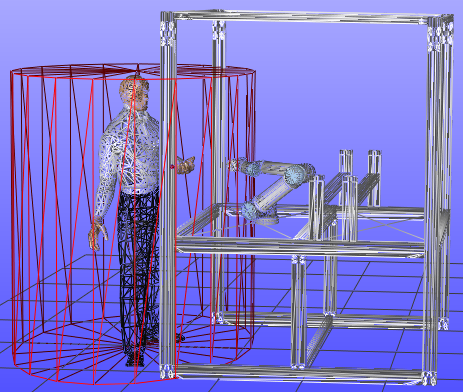
\includegraphics[scale=0.6]{images/introductionpicture.png}
 \caption{Scene to be used for planning. The red cylinder indicates the region
inside which the motion is to be constrained of the Universal Robot U1
}
 \label{fig:u1}
\end{figure}

Also note, that we both have produced two programs for this project. Jacobs program is used as a reference in this report. The another program is in the zip-file of the project.

\section{Relevant documents}
\begin{itemize}
\item See folder, "project3\_ PlanningOfSafeMotion/Jacob\_ code/", of Jacobs code, which also have been used in this report.
\item See folder, "project3\_ PlanningOfSafeMotion/mats\_ code/project3/",  of Mats code.
\item See textfile "project3\_ PlanningOfSafeMotion/mats\_ code/consolOutput.pdf", of console output of Mats code 
\item See document, "project3\_ PlanningOfSafeMotion/data.nb" of data generated by Mathematica
\end{itemize}